\documentclass{standalone}

\usepackage{tikz}

\begin{document}

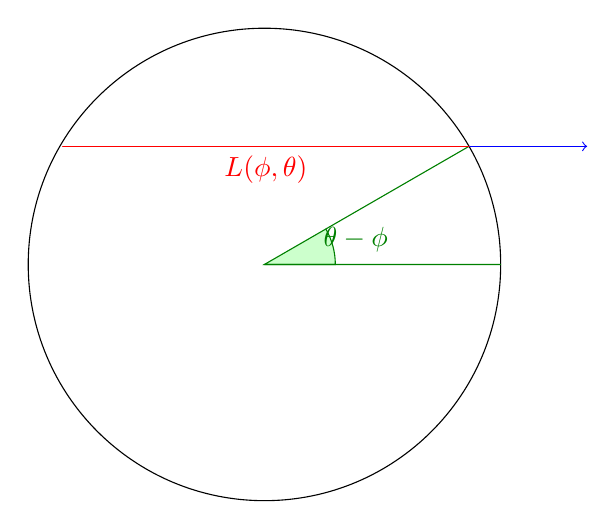
\begin{tikzpicture}[scale=3,cap=round]

    \colorlet{thetacolor}{green!50!black}
    \colorlet{phicolor}{blue}
    \colorlet{lcolor}{red}

    \draw (0,0) circle (1cm);

    \filldraw[fill=green!20,draw=thetacolor] (0,0) -- (3mm,0pt) arc(0:30:3mm);
    \draw (15:4mm) node[thetacolor] {$\theta-\phi$};

    \draw[thetacolor] (30:1cm) -- (0,0) -- (1cm, 0);

    \draw[->,phicolor] (30:1cm) -- +(0.5,0);

    \draw[lcolor] (30:1cm) -- node[below] {$L(\phi, \theta)$} +(-1.72, 0);

\end{tikzpicture}

\end{document}